In this chapter we develop a technique for estimating the distribution over failure trajectories for state-dependent sampling techniques. Having a distribution that approximates the distribution over failures allows us to sample a diverse set of likely failures as well as efficiently compute the probability of failure. We start by showing that a sampling distribution that is proportional to the probability of failure is an efficient proposal distribution, and is exactly the distribution over failures when the environment is deterministic. We then describe how to compute an estimate of the probability of failure using a Bellman equation. Through experiments in the gridworld and T-intersection environments, we show that even when the estimate of the probability of failure has a large amount of error, we still obtain an efficient proposal distribution compared to baseline techniques.

\section{Background}

% Why we care about a good failure distribution
- Falsification and most-likely failure analysis simply give examples but would not be able to certify the safety of a system because if they fail to produce examples we cannot say anything about why (since we are not search exhaustively)
-reference the figure
- talk about how if we ever wanted to improve our system we would train it on a diverse set of failures


%What. is wrong with existing approaches


- Importance sampling
- They don't use the state
- The state may be useful and it is especially important when the environment is stochastic or (just the initial conditions are)


% Outline our approach


\begin{figure*}
    \centering
    \begin{subfigure}[b]{0.45\textwidth}
        \centering
        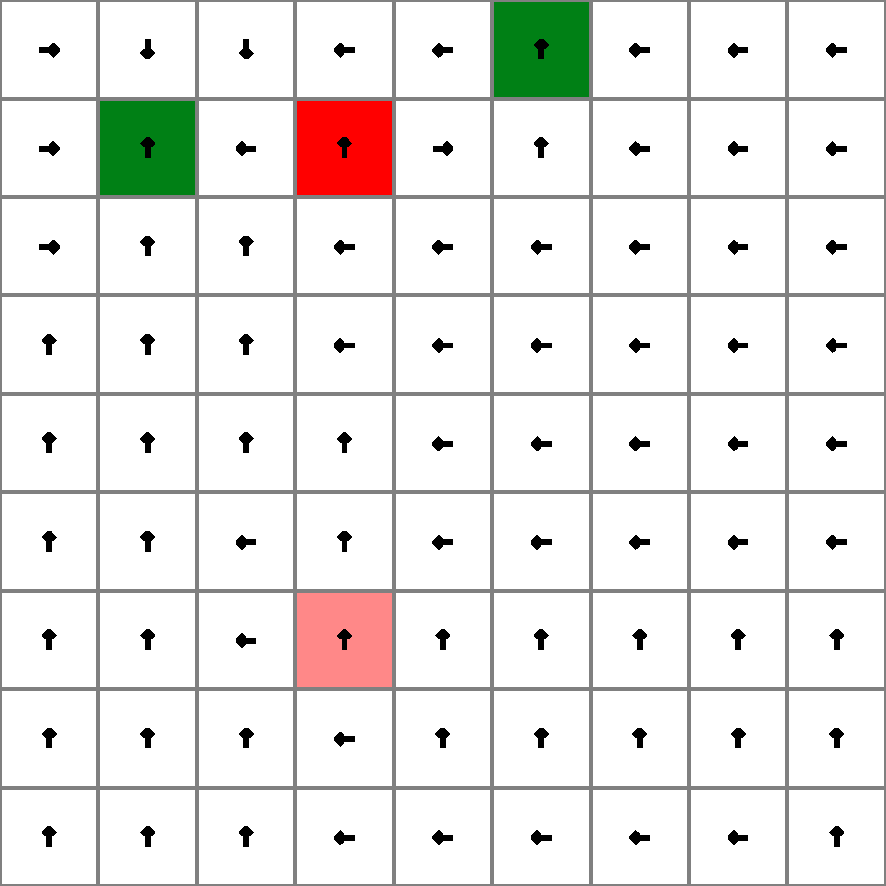
\includegraphics[width=\textwidth]{figures/distribution_over_failures/policy.pdf}
        \caption{Expert policy.}
        \label{fig:dof_policy}
    \end{subfigure}
    \hfill
    \begin{subfigure}[b]{0.45\textwidth}
        \centering
        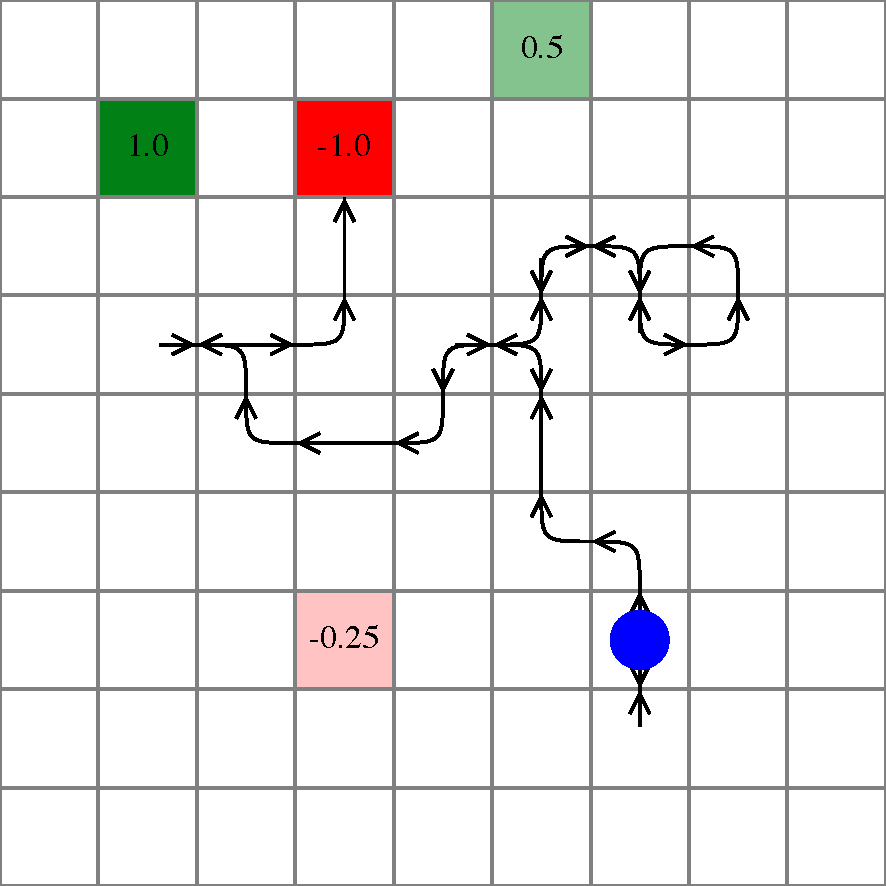
\includegraphics[width=\textwidth]{figures/distribution_over_failures/falsification_failure.pdf}
        \caption{Failure from falsification.}
        \label{fig:dof_falsification}
    \end{subfigure}
    \begin{subfigure}[b]{0.45\textwidth}
        \centering
        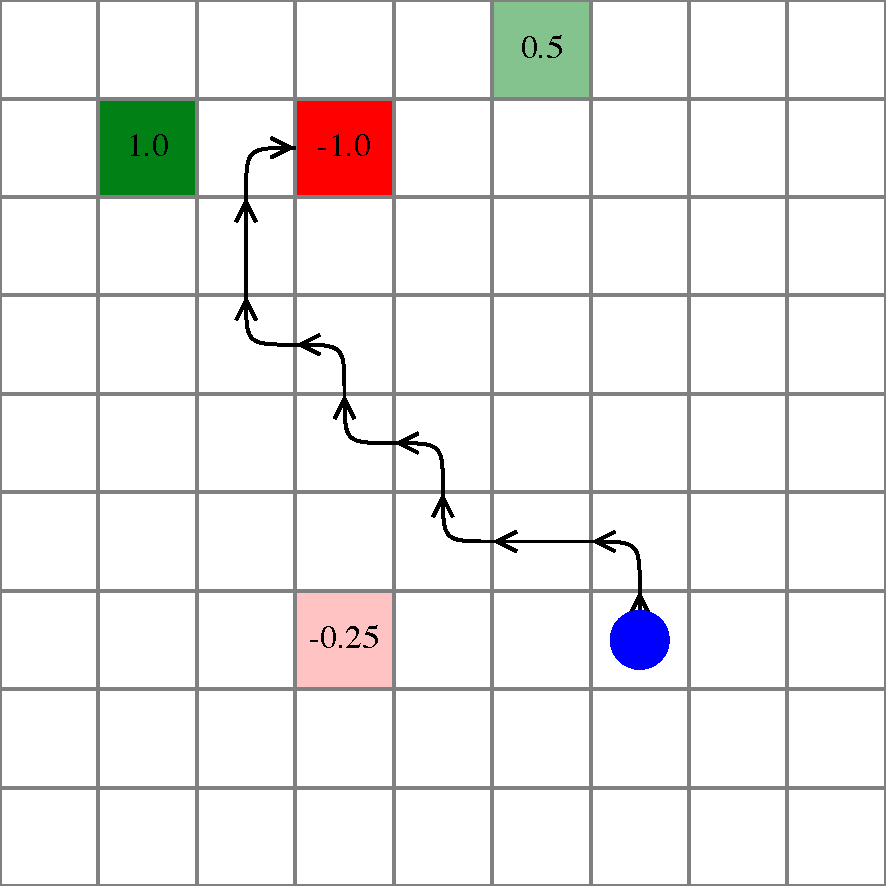
\includegraphics[width=\textwidth]{figures/distribution_over_failures/most_likely_failure.pdf}
        \caption{Most-likely failure.}
        \label{fig:dof_mostlikely_failure}
    \end{subfigure}
    \hfill
    \begin{subfigure}[b]{0.45\textwidth}
        \centering
        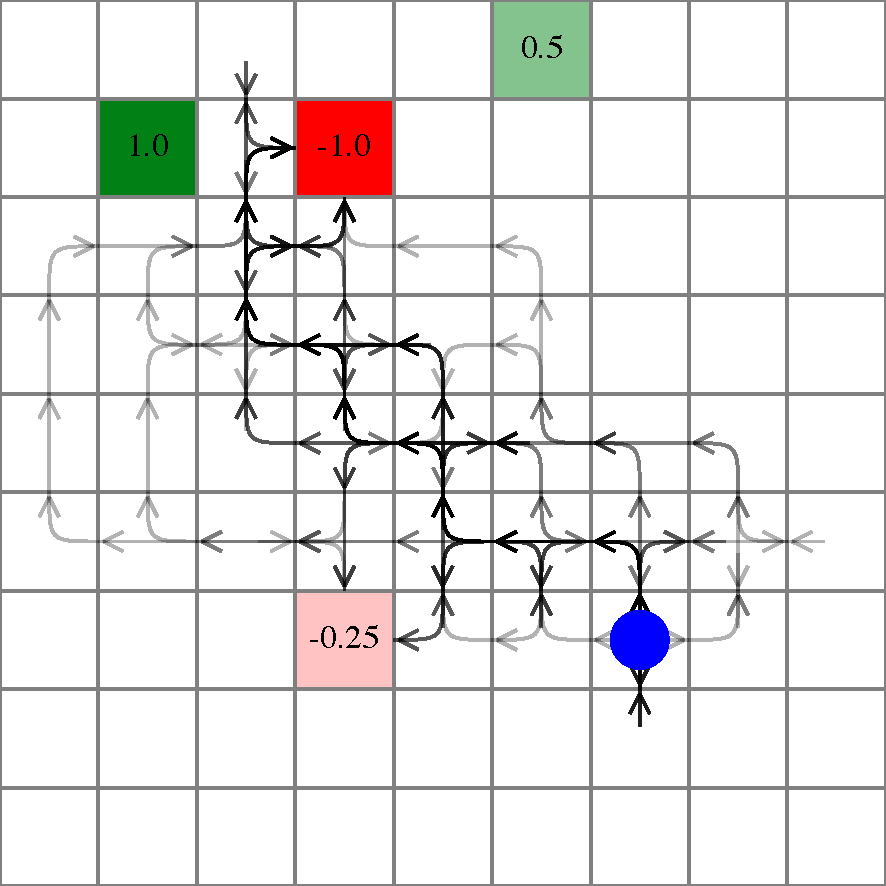
\includegraphics[width=\textwidth]{figures/distribution_over_failures/distribution_over_failures.pdf}
        \caption{Samples from failure distribution.}
        \label{fig:dof_dof}
    \end{subfigure}
    \caption{Comparison of safety validation tasks.}
    \label{fig:dof_comparison_safetytasks}
\end{figure*}





\section{Approach}

\todo{Discuss the challenge of designing a distribution where we can only control the disturbances $x$}

- Monte Carlo estimation

\subsection{State-dependent importance sampling}

% What are we trying to do:
The importance sampling approaches that were discussed in \cref{sec:is} construct a proposal distribution $q(\vec{x})$ to efficiently compute the probability of failure of a system. The downside to these approaches is that they do not consider the state of the environment when choosing each disturbance and therefore may not be using all of the available information. We wish to develop an importance sampling approach that can use the state of the environment to produce a more efficient proposal distribution. 


Let $\vec{\tau} = [s_0, x_1, s_1, \ldots x_{t_{\rm max}}, s_{t_{\rm max}}]$ be a trajectory of states and disturbances with probability $p(\vec{\tau})$. Without loss of generality we will assume a deterministic initial state $s_0$.  We wish to develop a proposal distribution $q(\tau)$ that can provide a good estimate of the probability of failure with the minimal number of samples. An unbiased estimator of the probability of failure from the initial state $s_0$ can be computed from $N$ independent sample trajectories $\vec{\tau}_i \sim q(\vec{\tau})$ as
\begin{equation}
\hat{P}_{\rm fail} = \frac{1}{N} \sum_{i=1}^N \frac{p(\vec{\tau}_i) \mathds{1}{\{ \vec{\tau}_i \not \in \psi \}}}{q(\vec{\tau}_i)} \text{,} \label{eq:pfail_estimator}
\end{equation}
where $\vec{\tau} \not \in \psi$ is equivalent to $\vec{s} \not \in \psi$ and represents a system failure. The number of samples we require depends upon the variance of this estimator which is given by
\begin{align}
\text{Var}_q\left[ \hat{P}_{\rm fail} \right] &= \frac{1}{N} \left( \mathbb{E}_q \left[\left(\frac{p(\vec{\tau}) \mathds{1}{\{ \vec{\tau} \not \in \psi \}}}{q(\vec{\tau})} \right)^2 \right] - \mathbb{E}_q\left[ \frac{p(\vec{\tau}) \mathds{1}{\{ \vec{\tau} \not \in \psi \}}}{q(\vec{\tau})}  \right]^2 \right) \\
&= \frac{1}{N} \left(\mathbb{E}_p \left[\frac{p(\vec{\tau}) \mathds{1}{\{ \vec{\tau} \not \in \psi \}}}{q(\vec{\tau})} \right] - P_{\rm fail}^2 \right)\label{eq:pfail_variance}
\end{align}
where have used the fact that $\mathbb{E}_q\left[ \hat{P}_{\rm fail}  \right] = P_{\rm fail}$. 

\subsection{Proposal distribution}

% Defining the proposal distribution
We now present a proposal distribution that it reduces the variance of $\hat{P}_{\rm fail}(s_0)$ compared to Monte Carlo sampling and is optimal in some situations. Define the disturbance policy
\begin{equation}
    q(x_t, \mid \vec{\tau}_{0:t-1}) = \frac{p(x_t \mid \vec{\tau}_{0:t-1}) P_{\rm fail}(\vec{\tau}_{0:t-1}, x_t)}{P_{\rm fail}(\vec{\tau}_{0:t-1})} \label{eq:disturbance_policy}
\end{equation}
where $\vec{\tau}_{0:t} = [s_0, x_1, s_1, \ldots, x_t, s_t]$ and $P_{\rm fail}(\vec{\tau}_{0:t})$ is the probability that the system fails under the distribution $p(\vec{\tau})$ after the sequence $\vec{\tau}_{0:t}$. To see that \cref{eq:disturbance_policy} is properly normalized we apply the recursive relationship between the probability of failure
\begin{equation}
    P_{\rm fail}(\vec{\tau}_{0:t-1}) = \sum_{x_t} p(x_t \mid \vec{\tau}_{0:t-1}) P_{\rm fail}(\vec{\tau}_{0:t-1}, x_t) \text{.}
\end{equation}
If we assume that states are sampled from the transition model $p(s_t \mid \vec{\tau}_{0:t-1}, x_t)$, then the resulting proposal distribution is
\begin{align}
    q(\vec{\tau}) &= \prod_{t=1}^{t_{\rm max}} \frac{p(x_t, s_t \mid \vec{\tau}_{0:t-1}) P_{\rm fail}(\vec{\tau}_{0:t-1}, x_t)}{P_{\rm fail}(\vec{\tau}_{0:t-1})} \\
    &= p(\vec{\tau}) \prod_{t=1}^{t_{\rm max}} \frac{P_{\rm fail}(\vec{\tau}_{0:t-1}, x_t)}{P_{\rm fail}(\vec{\tau}_{0:t-1})} \text{.} \label{eq:full_proposal}
\end{align}


%The following analysis assumes that the state and action spaces are discrete, but a similar results may be obtained by appropriately switching summations over states and actions to integrals.



Proposition 2 - The variance of failure probability estimate (\cref{eq:pfail_estimator}) under the proposal distribution defined in \cref{eq:full_proposal} is 
\begin{align}
    \text{Var}_q\left[ \hat{P}_{\rm fail} \right] &= \frac{P_{\rm fail}^2}{N} \left( \mathbb{E}_{p_{\tau \mid \mathds{1} \{\vec{\tau} \not \in \psi\}}}  \left[ \prod_{t=1}^{t_{\rm max}} \frac{p(s_t \mid \vec{\tau}_{0:t-1}, x_t, \mathds{1} \left\{ \vec{\tau} \not \in \psi \right\})}{p(s_t \mid \vec{\tau}_{0:t-1}, x_t)} \right] - 1 \right) \\
    &= \frac{P_{\rm fail}^2}{N} \left( \mathbb{E}_{p_{\tau \mid \mathds{1} \{\vec{\tau} \not \in \psi\}}}  \left[ \prod_{t=1}^{t_{\rm max}} \frac{P_{\rm fail}(\vec{\tau}_{0:t})}{P_{\rm fail}(\vec{\tau}_{0:t-1}, x_t)} \right] - 1 \right) \\
\end{align}

proof:
To show this, we can start by substituting \cref{eq:full_proposal} into \cref{eq:pfail_variance} to get
\begin{equation}
    \text{Var}_q\left[ \hat{P}_{\rm fail} \right] = \frac{1}{N} \left(\mathbb{E}_p \left[\mathds{1}\{ \vec{\tau} \not \in \psi \} \prod_{t=1}^{t_{\rm max}} \frac{P_{\rm fail}(\vec{\tau}_{0:t-1})}{P_{\rm fail}(\vec{\tau}_{0:t-1}, x_t)} \right] - P_{\rm fail}^2 \right) \label{eq:starting_variance_expression}
\end{equation}
Then, applying Bayes' rule we have 
\begin{equation}
    P_{\rm fail}(\vec{\tau}_{0:t}) = \frac{p(\vec{\tau}_{0:t} \mid \mathds{1} \left\{ \vec{\tau} \not \in \psi \right\}) P_{\rm fail}}{p(\vec{\tau}_{0:t})} \text{.}
\end{equation}
When substituted into the ratio term in \cref{eq:starting_variance_expression} we get
\begin{align}
    \prod_{t=1}^{t_{\rm max}} \frac{P_{\rm fail}(\vec{\tau}_{0:t-1})}{P_{\rm fail}(\vec{\tau}_{0:t-1}, x_t)} &= \prod_{t=1}^{t_{\rm max}} \frac{p(\vec{\tau}_{0:t-1} \mid \mathds{1} \left\{ \vec{\tau} \not \in \psi \right\}) p(\vec{\tau}_{0:t-1}, x_t)}{p(\vec{\tau}_{0:t-1}, x_t \mid \mathds{1} \left\{ \vec{\tau} \not \in \psi \right\}) p(\vec{\tau}_{0:t-1})} \\
    &= \prod_{t=1}^{t_{\rm max}} \frac{p(x_t \mid \vec{\tau}_{0:t-1})}{p(x_t \mid \vec{\tau}_{0:t-1}, \mathds{1} \left\{ \vec{\tau} \not \in \psi \right\})} \\
    &= \prod_{t=1}^{t_{\rm max}} \frac{p(x_t, s_t \mid \vec{\tau}_{0:t-1})p(s_t \mid \vec{\tau}_{0:t-1}, x_t, \mathds{1} \left\{ \vec{\tau} \not \in \psi \right\})}{p(x_t, s_t \mid \vec{\tau}_{0:t-1}, \mathds{1} \left\{ \vec{\tau} \not \in \psi \right\})p(s_t \mid \vec{\tau}_{0:t-1}, x_t)} \\
    &= \frac{p(\vec{\tau})}{p(\vec{\tau} \mid \mathds{1} \left\{ \vec{\tau} \not \in \psi \right\})} \prod_{t=1}^{t_{\rm max}} \frac{p(s_t \mid \vec{\tau}_{0:t-1}, x_t, \mathds{1} \left\{ \vec{\tau} \not \in \psi \right\})}{p(s_t \mid \vec{\tau}_{0:t-1}, x_t)} \\
    &= P_{\rm fail}\prod_{t=1}^{t_{\rm max}} \frac{p(s_t \mid \vec{\tau}_{0:t-1}, x_t, \mathds{1} \left\{ \vec{\tau} \not \in \psi \right\})}{p(s_t \mid \vec{\tau}_{0:t-1}, x_t)} \label{eq:simplified_ratio}
\end{align}
where we have used the fact $p(\vec{\tau} \mid \mathds{1} \left\{ \vec{\tau} \not \in \psi \right\}) =  p (\vec{\tau})/P_{\rm fail}$ to get \cref{eq:simplified_ratio}. Finally, we get the desired result by plugging \cref{eq:simplified_ratio} into \cref{eq:starting_variance_expression} and applying the identity

\begin{equation}
    \mathbb{E}_p \left[ \mathds{1} \{\vec{\tau} \not \in \psi\} f(\vec{\tau}) \right] = \mathbb{E}_p \left[ \mathds{1} \{\vec{\tau} \not \in \psi\} \right] \mathbb{E}_{p_{\vec{\tau} \mid \mathds{1} \{\vec{\tau} \not \in \psi\}}}  \left[ f(\vec{\tau}) \right] \text{.}
\end{equation}



\section{Estimating the Probability of Failure}

% In both the deterministic and stochastic settings, the problem of generating the distribution over failures or the optimal importance sampling distribution involves estimating the probability of failure $P_{\rm fail}(s)$.


\section{Experiments}

\section{Robustness to errors}

\section{Comparison of sampling techniques}

\section{Discussion}